\documentclass[12pt,a4paper]{article}
\usepackage[T2A]{fontenc}
\usepackage[utf8]{inputenc}
\usepackage[russian]{babel}
\usepackage{amsmath,amssymb}
\usepackage{geometry}
\usepackage{graphicx}
\usepackage{float}
\usepackage{booktabs}
\geometry{margin=2.2cm}

\title{Сравнение метаэвристических алгоритмов CSOA и DROA}
\author{}
\date{июнь 2026}

\begin{document}
\maketitle

\section*{Постановка}
Требовалось выбрать два метода из CSOA, DROA и TROA, сравнить их на одной функции и добавить PSO для сопоставления. Для сравнения выбраны CSOA и DROA, так как первый метод чередует поиск и преследование, а второй использует взаимодействие агентов через соседей.

В качестве тестовой задачи использована функция Экли:
\[
f(x)=-20\exp\left(-0.2\sqrt{\frac{1}{n}\sum_i x_i^2}\right)
-\exp\left(\frac{1}{n}\sum_i \cos(2\pi x_i)\right)+20+e,
\]
где $x\in[-5,5]^2$. Известный глобальный минимум равен $f(0,0)=0$.

\section*{Кратко о методах}
В CSOA агент находится либо в режиме поиска, либо в режиме преследования. В режиме поиска строится несколько локальных кандидатов; в режиме преследования скорость обновляется в направлении лучшей найденной точки:
\[
v_i^{t+1} = v_i^t + c r (x^{best} - x_i^t), \qquad x_i^{t+1}=x_i^t+v_i^{t+1}.
\]

В DROA шаг агента складывается из разделения, выравнивания, сцепления, притяжения к пище и удаления от врага:
\[
\Delta X^{t+1} = sS+aA+cC+fF+eE+w\Delta X^t.
\]
В реализации пищей считается лучшая найденная точка, врагом -- худший агент текущей популяции.

PSO добавлен как базовый метод:
\[
v_i^{t+1} = wv_i^t+c_1r_1(p_i^{best}-x_i^t)+c_2r_2(g^{best}-x_i^t).
\]

\section*{Параметры}
\begin{center}
\begin{tabular}{lr}
\toprule
Параметр & Значение \\
\midrule
Число агентов & 45 \\
Число итераций & 160 \\
CSOA: SMP & 5 \\
CSOA: SRD & 0.22 \\
CSOA: MR & 0.22 \\
DROA: радиус соседства & 0.08--0.65 диагонали \\
PSO: $c_1$, $c_2$ & 1.55; 1.65 \\
\bottomrule
\end{tabular}
\end{center}

\section*{Результаты}
\begin{center}
\begin{tabular}{lrrrr}
\toprule
Метод & $x_1$ & $x_2$ & $f(x)$ & расстояние до $(0,0)$ \\
\midrule
PSO & 0.000000 & 0.000000 & 0.000000 & 0.000000 \\
CSOA & -0.000319 & -0.000804 & 0.002468 & 0.000865 \\
DROA & 0.011198 & 0.008554 & 0.045137 & 0.014091 \\
\bottomrule
\end{tabular}
\end{center}

Все методы приблизились к известному минимуму. На данной постановке PSO сходится быстрее, CSOA стабильно уточняет решение через локальные пробы, DROA сильнее зависит от радиуса соседства и веса притяжения к лучшей точке.

\section*{Графики}
\begin{figure}[H]
\centering
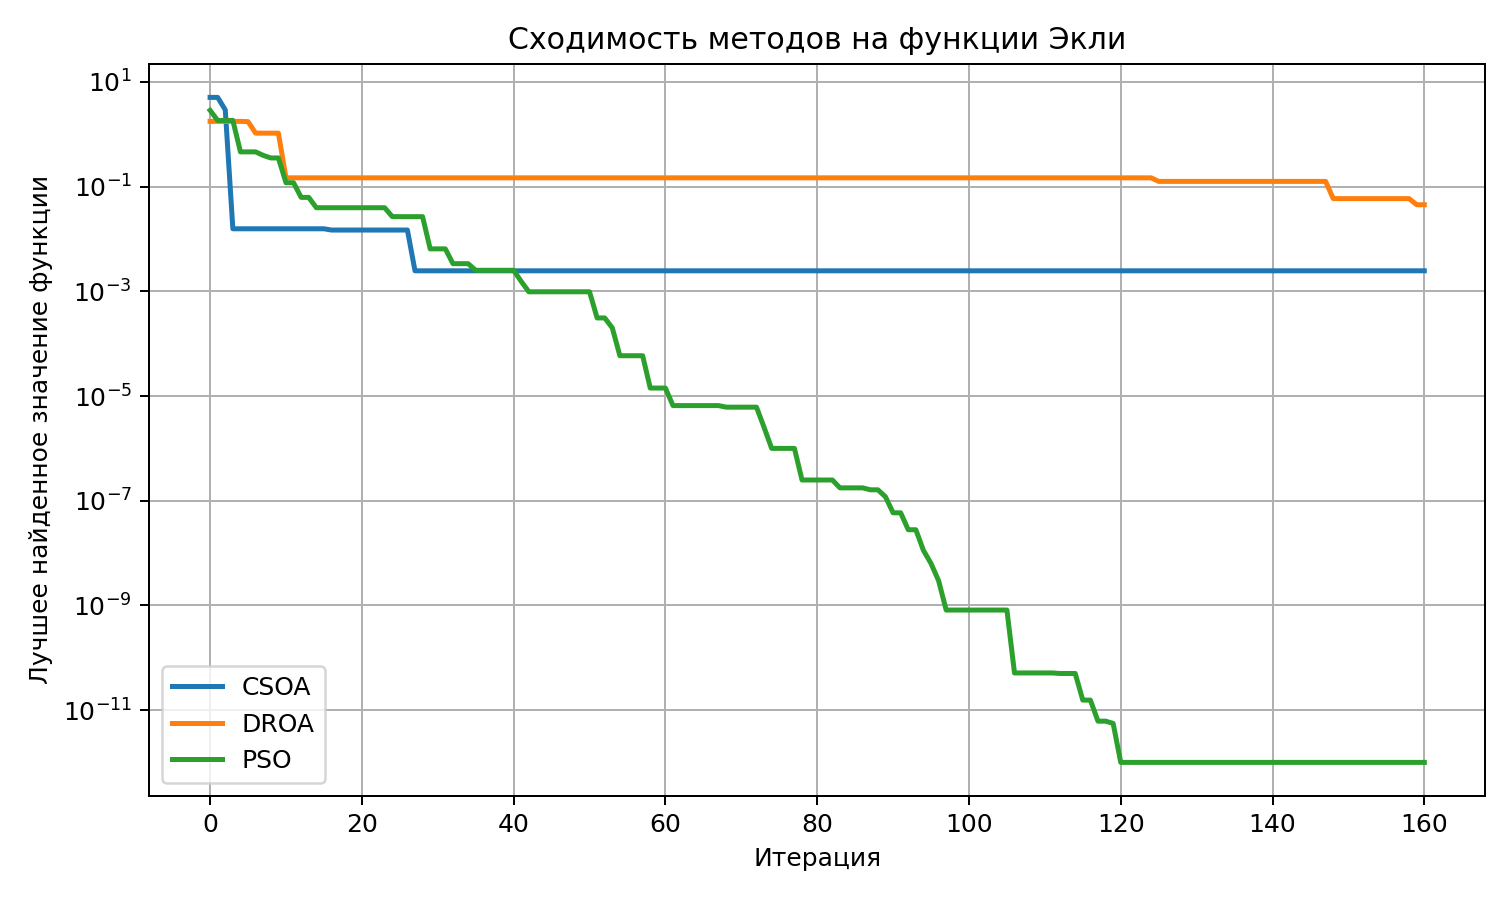
\includegraphics[width=0.88\textwidth]{graphs/convergence_comparison.png}
\caption{Лучшее найденное значение функции от номера итерации.}
\end{figure}

\begin{figure}[H]
\centering
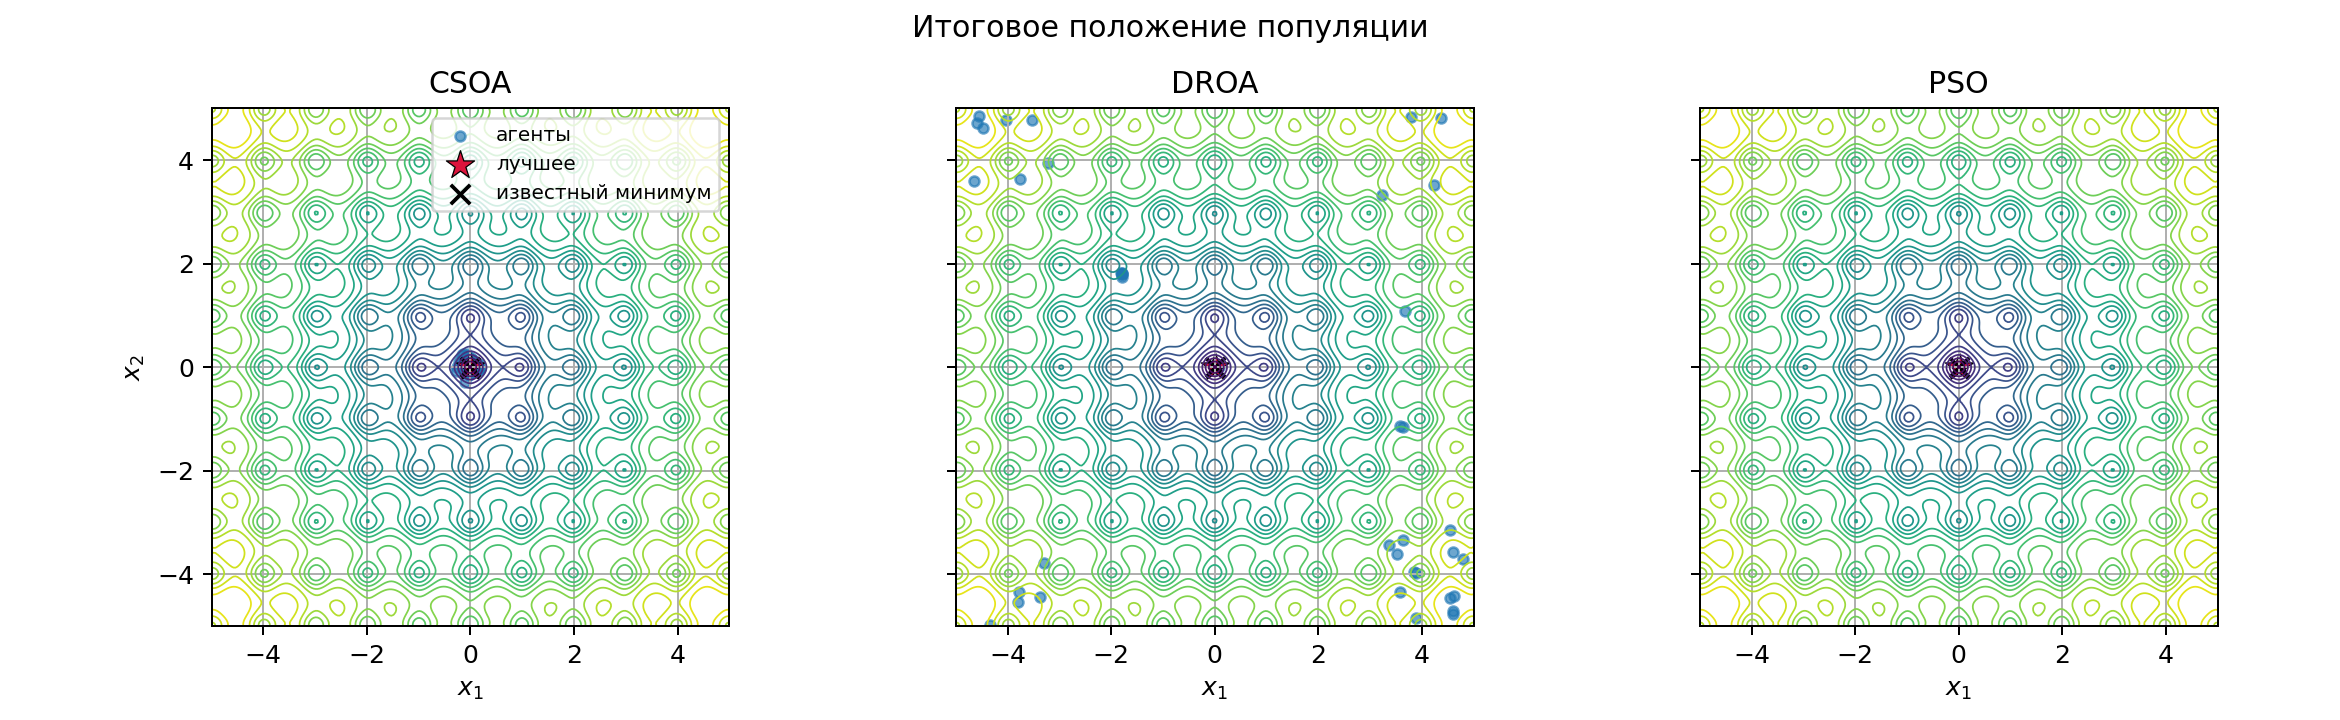
\includegraphics[width=0.96\textwidth]{graphs/final_positions_comparison.png}
\caption{Итоговое положение популяций на линиях уровня функции.}
\end{figure}

\begin{figure}[H]
\centering
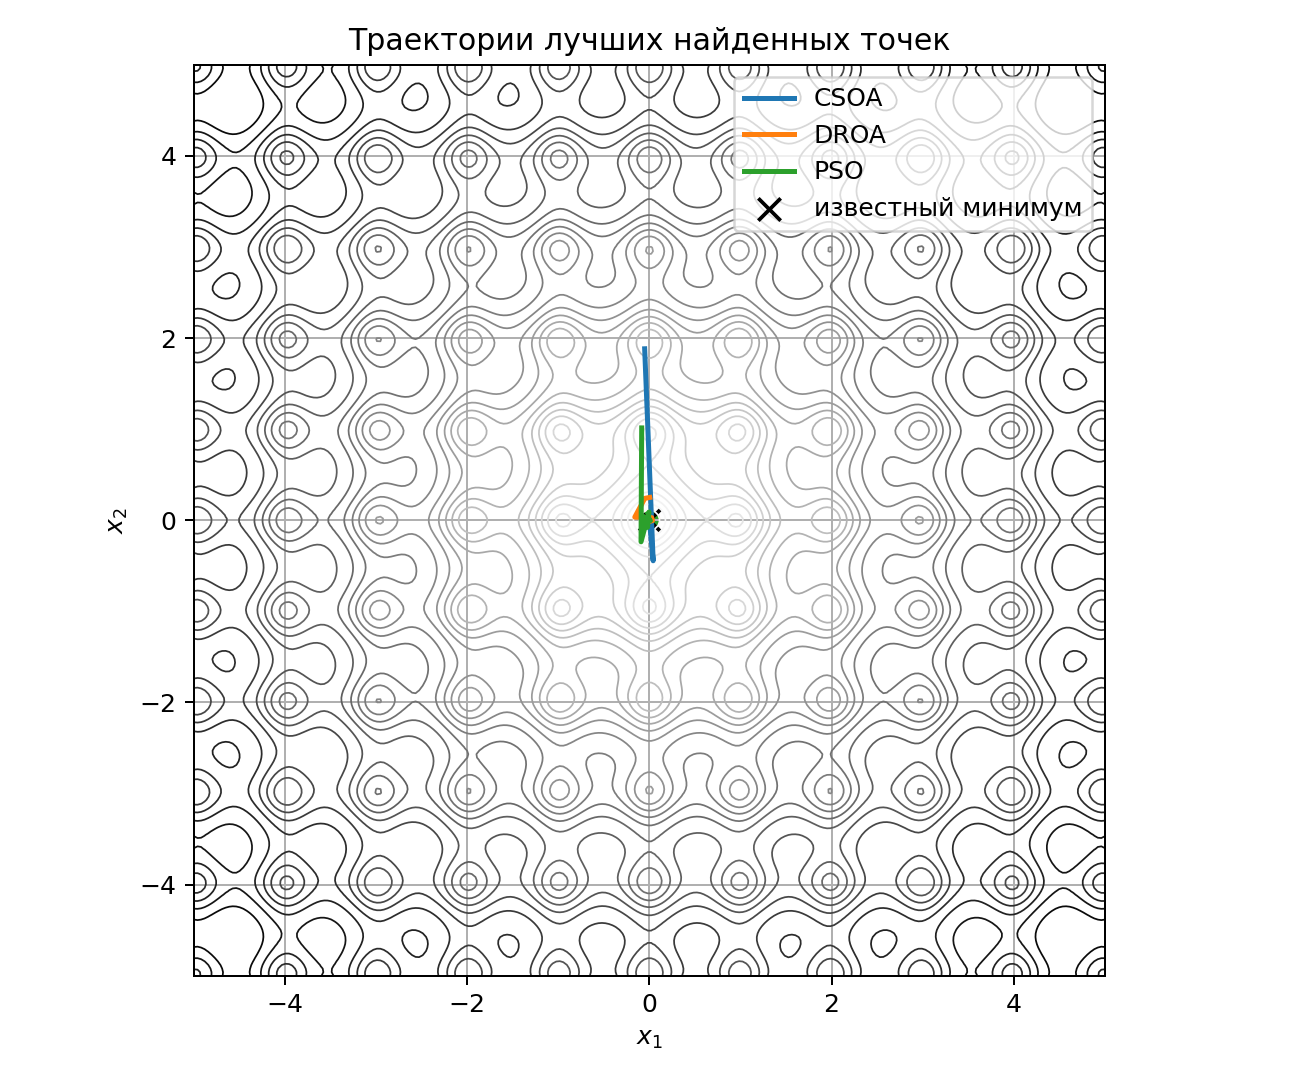
\includegraphics[width=0.76\textwidth]{graphs/best_paths_comparison.png}
\caption{Траектории лучших найденных точек.}
\end{figure}

\begin{figure}[H]
\centering
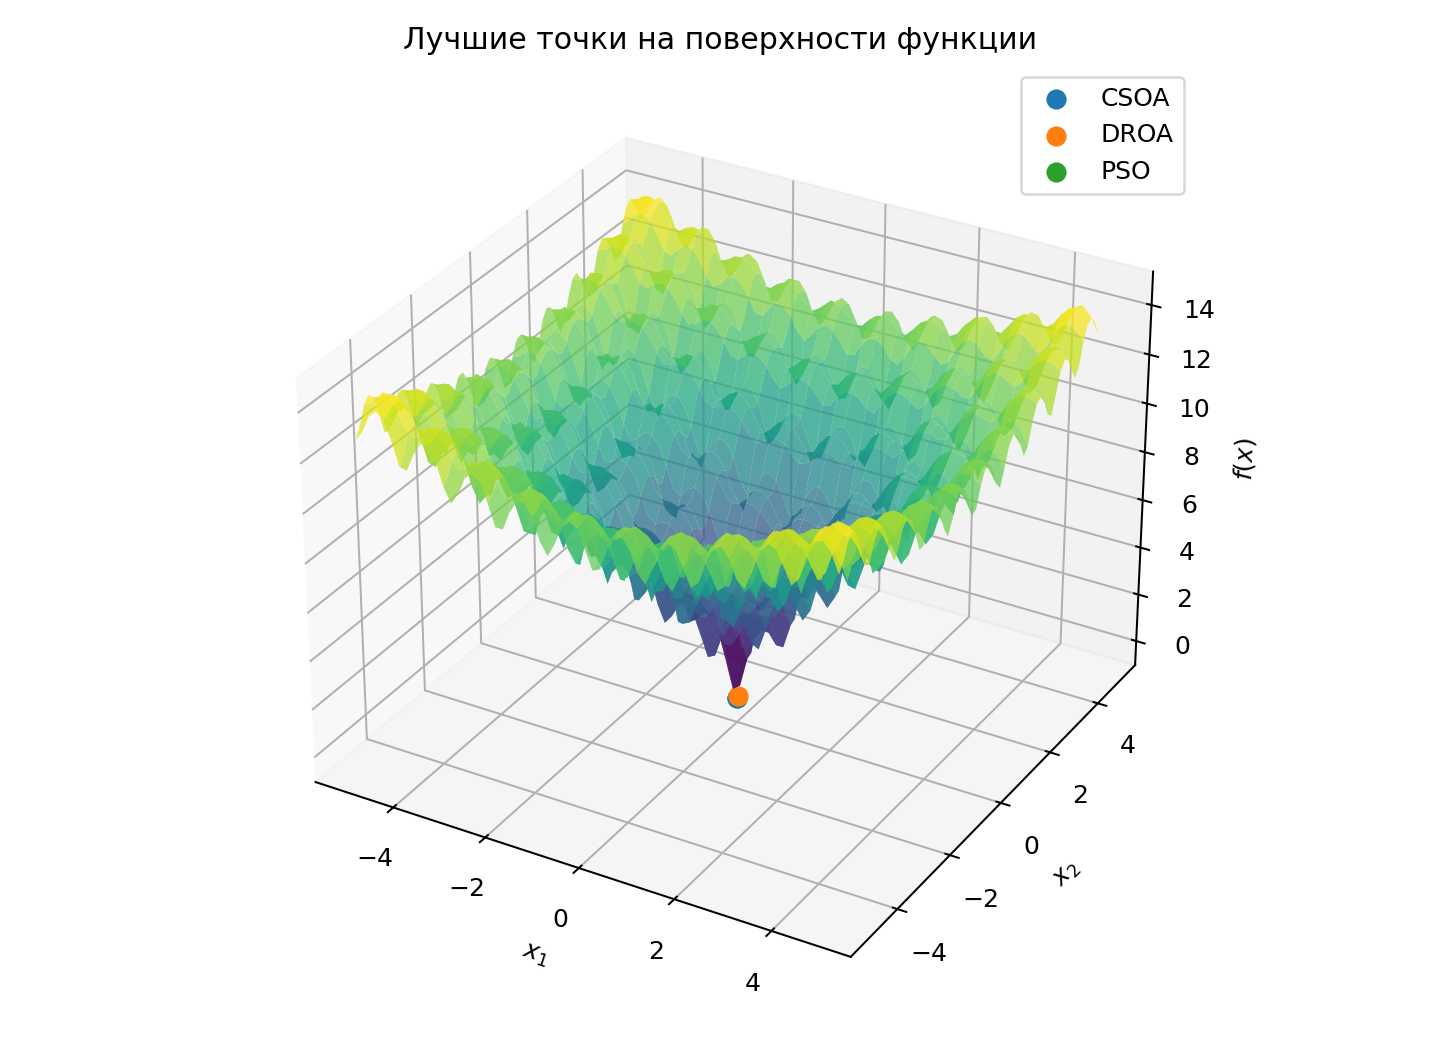
\includegraphics[width=0.78\textwidth]{graphs/surface_best_points.png}
\caption{Лучшие точки на поверхности функции.}
\end{figure}

\section*{Вывод}
Для выбранной функции все три алгоритма нашли точки около глобального минимума. PSO оказался самым быстрым на гладкой двумерной задаче, но CSOA и DROA также дают рабочую схему глобального поиска. Код в ноутбуке позволяет заменить функцию и параметры без изменения структуры эксперимента.

\end{document}
